%%%%%%%%%%%%%%%%%%%%%%%%%% 
% vše co následuje bude uvedeno v přílohách
\appendix	
\printnomenclature
\label{apx:zkratky}
\chapter{Ukážka dát}

\lstinputlisting[language=JavaScript,
			caption=Ukážka CDC správy odoslanej Debeziom,
            label=code:schemaExample]
            {code/2/CDC_message_structure.json}

\chapter{Ukážky zdrojových kódov}

\lstinputlisting[language=Java2,
			caption=Parsovacie metódy DDL parserov, 
            label=code:parseMethod]
            {code/3/parseMethod.java}

\lstinputlisting[language=Java2,
			caption=Implementácia parseNextStatement metódy v MySqlDdlParser, 
            label=code:mysqlParseNextStatement, float]
            {code/3/mysqlParseNextStatement.java}

\lstinputlisting[language=Java2,
			caption=Implementácia parseCreateTable metódy v MySqlDdlParser, 
            label=code:parseCreateTable,
            float,floatplacement=H,
            basicstyle=\small]
            {code/3/parseCreateTable.java}
           
\lstinputlisting[language=Java2,
			caption=Implementácia metódy na vymazanie tabuliek, 
            label=code:removeTablesByDatabase, float]
            {code/6/removeTablesByDatabase.java}
            
\lstinputlisting[language=Java2,
			caption=Inicializácia komponenty DataTypeResolver, 
            label=code:registerDataTypes, float]
            {code/6/registerDataTypes.java}

\lstinputlisting[language=Java2,
			caption=Implementácie rozhodovacieho algoritmu komponenty DataTypeResolver, 
            label=code:resolveDataType, float]
            {code/6/resolveDataType.java}

\chapter{Postup inštalácie ANTLR nástroja}

\lstinputlisting[caption=Kroky inštalácie ANTLR nástroja pre Windows, 
            label=install:windows]
            {code/5/antlr_install.tex}

\lstinputlisting[caption=Kroky inštalácie ANTLR nástroja pre Linux/Mac OS, 
            label=install:linux]
            {code/5/antlr_install.sh}


\chapter{Obsah přiloženého CD}
\begin{itemize}
   \item{\textit{prototyp}} (spustitený soubor *JAR* vytvořené prototypové implementace obsahující všechny závislosti)
   \item{\textit{DP\_Moravec\_Jakub\_2018}} (text diplomové práce ve formátu \textit{PDF})
   \item{\textit{dokumentace}} (dokumentace prototypové implementace)
      \begin{itemize}
         \item{\textit{api\_javadoc}} (\textit{javadoc} dokumentace navrženého \textit{API} perzistentní vrstvy)
         \item{\textit{diagramy}} (diagramy obsažené v diplomové práci)
      \end{itemize}
   \item{\textit{zdrojove\_kody}}
      \begin{itemize}
         \item{\textit{prototyp}} (zdrojové kódy prototypové implementace navržené architektury)
         \item{\textit{PoC}} (zdrojové kódy dvou \textit{PoC} implementací provedených v rámci sekce \ref{sec:des_transactions})
         \item{\textit{diplomova\_prace}} (zdrojové kódy diplomové práce ve formátu \textit{TEX})
      \end{itemize}
   \item{\textit{knihovny}} (privátní knihovny \textit{Manta FLow} nutné k sestavení prototypové implementace)
   \item{\textit{vzorove\_vstupy}} (vzorové vstupní soubory pro prototypovou implementaci)
   \item{\textit{README.MD}} (soubor definující požadavky k sestavení, spuštění a korektní funkčnosti prototypové implementace)
\end{itemize}

\textbf{\large Tato příloha je povinná pro každou práci. Každá práce musí totiž obsahovat přiložené CD. Viz dále.}
Může vypadat například takto. Váš seznam samozřejmě bude odpovídat typu vaší práce. (viz \cite{infodp}):
\begin{figure}[h]
\begin{center}
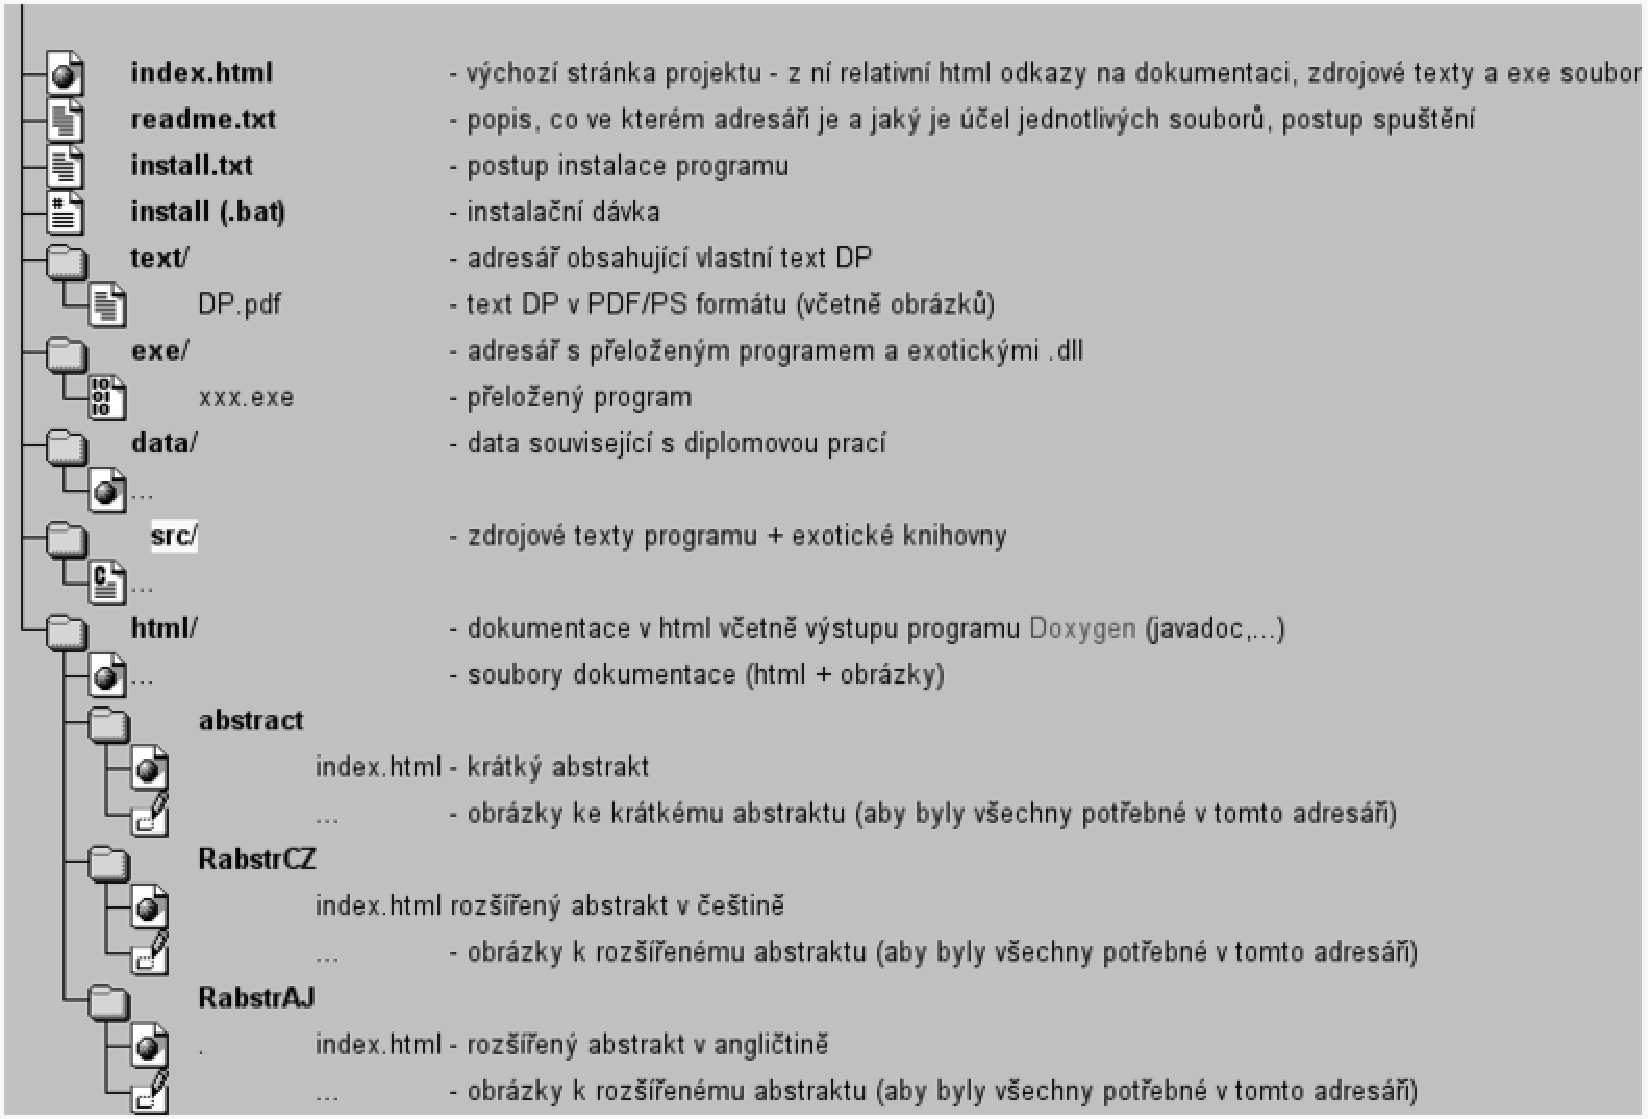
\includegraphics[width=14cm]{figures/seznamcd}
\caption{Seznam přiloženého CD --- příklad}
\label{fig:seznamcd}
\end{center}
\end{figure}
Na GNU/Linuxu si strukturu přiloženého CD můžete snadno vyrobit příkazem:\\ 
\verb|$ tree . >tree.txt|\\
Ve vzniklém souboru pak stačí pouze doplnit komentáře.

Z \textbf{README.TXT} (případne index.html apod.)  musí být rovněž zřejmé, jak programy instalovat, spouštět a jaké požadavky mají tyto programy na hardware.

Adresář \textbf{text}  musí obsahovat soubor s vlastním textem práce v PDF nebo PS formátu, který bude později použit pro prezentaci diplomové práce na WWW.
